
In the remainder of this thesis we will be most interested in certain non-trivial aspects that gravitational interactions exhibit, which are quantum in origin and moreover single out gravity from the rest of the interactions observed in Nature. However, in order to properly understand what makes gravity so special, it is crucial to have in mind which properties are actually shared by other fundamental forces. In this regard, the most interesting statement concerns the fact that both kind of interactions can be accommodated --- at low enough energies --- within the same theoretical framework, namely that of \emph{effective field theory} (EFT).

Indeed, we are by now familiar with the idea of \emph{separation of scales}. This concept turns out to be crucial in our modern understanding of physics, acting moreover as a useful organizing principle. It posits that physics itself can be essentially understood in an independent manner at each energy scale (or more accurately regime), therefore avoiding the important but subtle question of what is happening at much higher energies (equivalently very short distances), which cannot be resolved by our experimental apparatus. A clear example of this is the theory of hydrodynamics, which correctly describes how certain fluids (e.g., water) flow in streams or rivers, without caring too much about the details of the processes that occur at the molecular or even (sub-)atomic level. In a sense, what we do is isolate the relevant degrees of freedom that are needed in order to describe some physical phenomena and then use an effective `coarse-grain' description. Of course, this does not mean that the physics at higher energies does not matter, since after all the low energy theory may be, in principle, retrieved from this more fundamental description. 

Furthermore, one can argue that the conclusion drawn in the previous paragraph is in fact unavoidable. More precisely, if we want our effective description to be compatible with \emph{(i)} Lorentz invariance, \emph{(ii)} quantum mechanics (causality, unitarity, crossing symmetry) and \emph{(iii)} locality (in the form of cluster decomposition), we must resort to quantum field theory \cite{Weinberg:2016kyd, Weinberg:2021exr}. Therefore, the EFTs we usually have to deal with are defined as a path integral
%
\beq
\mathcal{Z}_{\Lambda} = \int \mathcal{D} \Phi \mathcal{D} \Psi \mathcal{D} A \mathcal{D} g\ e^{\text{i} S_{\Lambda} \left[ \Phi,\, \Psi,\, A,\, g\right]/\hbar}\, ,
\label{eq:EFTpathintegral}
\eeq
%
where the action functional includes terms of the form (assuming the existence of some lagrangian description) 
%
\beq
\begin{aligned}
    S_{\Lambda} \left[ \Phi,\, \Psi,\, A,\, g\right] = \int \dd^4x \sqrt{-g} \Bigg( & \frac{1}{2 \kappa_4^2} \left(\mathcal{R} - 2 \Lambda_{\rm c.c.} \right) - \frac{1}{4} F^2 - \frac{1}{2} \left(\partial \Phi \right)^2 + \text{i} \bar{\Psi}  \slashed{\partial} \Psi\\
    &- V(\Phi) + \mathcal{Y}_{\rm yuk} \Phi \bar{\Psi} \Psi + \ldots\Bigg)\, ,
\end{aligned}
\label{eq:EFTaction}
\eeq
%
with $\Phi(x)$ describing scalar degrees of freedom, $\Psi^{\alpha}(x)$ is Grassmann-valued, $A_{\mu}(x)$ accounts for gauge interactions, $g_{\mu \nu} (x)$ denotes the gravitational field and the ellipsis indicates any further local higher-dimensional operator that may appear in the action. The subscript `$\Lambda$' both in \eqref{eq:EFTpathintegral} and \eqref{eq:EFTaction} signify that the path integral is meant to be restricted to field variations which probe energy scales no greater than the ultra-violet (UV) cut-off $\Lambda$, beyond which new physics (in the form of e.g., very massive degrees of freedom) may arise. From this perspective, it is clear that gravity is not much different than other interactions appearing in the effective action $S_{\Lambda}$, and in fact one must include gravitational degrees of freedom in the path integral so as to account for classical dynamical phenomena such as gravitational waves \cite{GW1,GW2}.

The actual difference between gravity and say (non-)Abelian gauge theories becomes manifest when studying how the amplitudes of physical processes behave as we vary the energy of the external particles. Indeed, the gravitational coupling $\kappa_4$ can be related to the more familiar Newton's constant $G_N$ as follows
%
\beq
 \kappa_4^2 = 8 \pi G_N\, ,
\label{eq:gravconstant4d}
\eeq
%
which has units of $[E]^{-2}$ in four dimensions and is extremely small. As a consequence, we deduce that General Relativy (GR) is \emph{non-renormalizable}, thus implying that it is a priori more sensitive to the relevant UV physics than its renormalizable counterparts. However, when viewed from the prism of effective field theory, this simply means that one can organize the theory into an energy expansion which \emph{must} include higher-curvature as well as higher-dimensional operators, whose form is moreover highly constrained by the symmetries of the theory (i.e. general covariance). Furthermore, given the smallness of $G_N$ at ordinary energies, one deduces that gravity is very well-suited for perturbation theory, as long as we remain within its range of applicability.

The aim of this chapter is to revisit these issues and try to pinpoint, from the perspective of a low energy observer, what would be the precise regime of validity of any EFT weakly coupled to Einstein gravity. In other words, the main question that will occupy us in the following is what is the maximum energy cut-off $\Lambda$ of any such effective description. The discussion is thus organized as follows. In Section \ref{s:genrelEFT} we will propose a first potential candidate for the quantum gravity cut-off $\LQG$, based on our experience with other non-remormalizable theories, such as the Fermi theory of weak interactions or the chiral lagrangian in quantum chromo-dynamics (QCD). There we also elaborate on the EFT-like expansion that one would expect to arise within these gravitational theories, since it will play an important role in Chapter \ref{ch:Higherdimops} of this thesis. Later on, in Section \ref{s:speciesmotivation} we reconsider the validity of this answer in the presence of a large amount of light degrees of freedom, both from a perturbative and non-perturbative perspective. In particular, this introduces certain puzzles related to (the minimal) black hole entropy, and leads to a seemingly different proposal for $\LQG$. Finally, in Section \ref{s:speciesscale}, we elaborate on the possibility that the energy scale introduced in Section \ref{s:speciesmotivation} be precisely identified with the quantum gravity cut-off. We also argue that this observation may have profound impact when embedded into the Swampland program, as we investigate more thoroughly in Parts \ref{part:StringTheoryTests} and \ref{part:pattern} of the thesis.

Most of the material included in this chapter is based on results existing in the literature, whilst the rest has been taken from the publications \cite{Castellano:2022bvr, Castellano:2023aum}. We will include the appropriate references accordingly, so as to distinguish the original contributions in this work from already known results.   

\section{General relativity as an effective field theory}
\label{s:genrelEFT}	

In this section we review what is the typical structure of non-renormalizable EFTs in order to hopefully extract some general lessons regarding their predictive power. To do so, we briefly consider in Section \ref{ss:nonrenormalizableEFTs} a simple and familiar example, namely 4-Fermi theory. Subsequently, in Section \ref{ss:basics} we apply these ideas in the context of gravitational interactions. The discussion here is based on refs. \cite{Burgess:2020tbq,Donoghue:1994dn,Donoghue:2022eay} (see also references therein), to which we refer the reader interested in more details. %\AC{quizá dar más refs a EFT reviews}

\subsection{Non-renormalizable field theories}
\label{ss:nonrenormalizableEFTs}

For any given effective field theory, what is (non-)renormalizable strongly depends on the dimension of the target spacetime. Hence, in order to be as general as possible (and with an eye to future applications in the context of string theory), let us consider here some $d$-dimensional EFT with an action functional of the form   
%
\beq
\begin{aligned}
    S_{\rm EFT} = \int \dd^dx \left( \mathcal{L}_{\rm ren} + \mathcal{L}_{\cancel{\rm ren}}\right)\, ,
\end{aligned}
\label{eq:EFTactionII}
\eeq
%
where $\mathcal{L}_{\rm ren}$ ($\mathcal{L}_{\cancel{\rm ren}}$) denotes the (non-)renormalizable lagrangian density. On the one hand, $\mathcal{L}_{\rm ren}$ typically includes local operators whose classical mass dimension is smaller than or equal to $d$, such as kinetic or mass terms as well as the first few low-lying interactions, i.e. scalar potentials, Yukawa or gauge interactions, etc. (c.f. eq. \eqref{eq:EFTaction}). Their significance lies in the fact that they capture the most \emph{relevant} physics (in the Wilsonian sense) at low energies. Moreover, even if they do not provide for the full UV complete theory, their physical predictions are shielded from the very high energy degrees of freedom, which may enter when computing quantum (e.g., loop) corrections in \eqref{eq:EFTpathintegral}. This follows from the Appelquist-Carazzone theorem \cite{Appelquist:1974tg}, which ensures that all such effects can be either effectively encoded into the `running' of a finite number of physical parameters that enter into the original lagrangian and can be measured in experiments (i.e. the masses and couplings of the theory), or are rather highly suppressed at low energies. Hence, such renormalizable theories are very appealing from the theoretical point of view, since one can in principle make an infinite number of predictions once a few coupling constants have been determined experimentally. A canonical example of this class of theories is quantum electro-dynamics (QED) in four dimensions \cite{Feynman:1949zx, Feynman:1950ir}
%
\beq
\begin{aligned}
    S_{\rm QED} \left[ A, \psi\right] = \int \dd^4x \left( -\frac{1}{4 e^2} F^{\mu \nu} F_{\mu \nu} + \bar{\psi} \left( \text{i} \slashed{D} -m\right) \psi\right)\, ,
\end{aligned}
\label{eq:QED}
\eeq
%
where $F_{\mu \nu} = \partial_{\mu} A_{\nu}- \partial_{\nu} A_{\mu}$ denotes the field strength of the photon, $D_{\mu} = \partial_{\mu} - \text{i} A_{\mu}$ is the $\mathsf{U(1)}$ covariant derivative and $e$ determines the gauge coupling constant. This theory is interacting, describes the electromagnetic force observed in our world and offers many interesting predictions. Among them one finds effective photon interactions, which appear to be forbidden at the classical level but are instead generated by quantum corrections due to the electron-positron field $\psi (x)$. In fact, some of these can be calculated exactly at one-loop, yielding the following local lagrangian due to Heisenberg (see e.g., \cite{Schwartz:2014sze})
%
\beq
\begin{aligned}
    \mathcal{L}_{\rm EH}\, =\, \frac{e^2}{360 \pi m^4} \left[ \left( F^{\mu \nu} F_{\mu \nu} \right)^2+ \frac74 \left( F^{\mu \nu} \tilde{F}_{\mu \nu}\right)^2\right]\, ,
\end{aligned}
\label{eq:Euler-Heisenberg}
\eeq
%
where $\tilde{F}_{\mu \nu} = \frac12 \epsilon_{\mu \nu \rho \sigma} F^{\rho \sigma}$ is the Hodge dual field strength.

On the other hand, the non-renormalizable piece frequently consists in an infinite number of local operators of mass dimension $n>d$, as follows
%
\beq
\begin{aligned}
    \mathcal{L}_{\cancel{\rm ren}}\, \supset\, \sum_{n>d}^{\infty} c_n \frac{\mathsf{O}_n \left( \Phi,\, \Psi,\, \ldots\right)}{\Lambda_{\rm UV}^{n-d}}\, ,
\end{aligned}
\label{eq:nonrenlagrangian}
\eeq
%
where we have absorbed the dimensions into some energy scale $\Lambda_{\rm UV}$, thus leaving us with a set of \emph{Wilson coefficients} $\{c_n\}$, which are dimensionless parameters generically of order 1 (or at least not parametrically large/small except possibly for a few of them). Notice that the introduction of the same dimensionful quantity $\Lambda_{\rm UV}$ for each operator in \eqref{eq:nonrenlagrangian} can be done without any loss of generality. The non-trivial statement concerns the order of magnitude of the expansion coefficients, and the fact that they become roughly of the same order implies that they agree on the maximum energy scale at which the theory can be trusted, namely the UV cut-off discussed around eq. \eqref{eq:EFTaction}. That this indeed happens for any existing non-renormalizable EFT has not been proven rigorously, but rather may be regarded as a general expectation coming from our field theory experience and is moreover supported by examples, see below. Let us also note that the terms appearing in $\mathcal{L}_{\cancel{\rm ren}}$ are usually referred to as \emph{irrelevant} operators, since their contribution to physical processes at low enough energies (i.e. well below $\Lambda_{\rm UV}$) is negligible,\footnote{Of course, this is true as long as the renormalizable piece contributes to the process under consideration, since otherwise it is the non-renormalizable operator the one providing for the leading order term in the energy expansion. A well-known example being the case of dimension-6 operators allowing for the proton decay in supersymmetric grand unified theories (see e.g., \cite{Raby:2002wc}).} whereas they become important in the ultra-violet regime --- being moreover sensitive to the UV completion of the theory.

From our previous discussion, one could be tempted to conclude that indeed non-renormalizable field theories seem to be less appealing than their renormalizable counterparts. However, the modern Wilsonian understanding of effective field theories actually flips this logic around and suggests that it is indeed the non-renormalizable EFTs the ones that are most interesting as well as predictive. The reason for this is twofold: first, from the `top-down' perspective, it may be sometimes useful to not bother about all the details and complications associated to the UV complete theory, and just construct --- using e.g., symmetry principles --- a simpler EFT for the relevant light degrees of freedom, which typically is of the non-renormalizable type and yields the same answers. Second, from the `bottom-up' point of view, these theories oftentimes predict their own failure, in the sense that they tend to organize into some energy expansion in terms of the UV cut-off $\Lambda_{\rm UV}$ as in \eqref{eq:nonrenlagrangian}, which signals the appearance of new physics around that scale which cannot be accounted for by the original theory. In the following, we will illustrate these ideas using perhaps the most simple example of a non-renormalizable EFT (at least in the context of particle physics), namely the 4-Fermi effective theory of weak interactions.


\subsubsection*{Example: Fermi theory of weak interactions}

The effective theory of weak interactions was originally introduced by Fermi \cite{Fermi:1934hr} as an extension of QED, in order to account for certain phenomena (like $\beta$-decay) which could not be explained within the theoretical framework existing at that time. It was moreover constructed purely from a `bottom-up' perspective, since the non-Abelian character of the underlying gauge theory was not known yet, and indeed it is very practical for all purposes as long as we want to describe physical processes involving weak interactions (e.g., muon decay) at energies well below the mass of the $W$ boson. However, in order to better connect with our previous discussion, we will derive this effective theory from the `top-down', i.e. starting with the Standard Model (SM) of particle physics.

As we now know, the weak interactions are mediated by the $W^{\pm}$ and $Z^0$ bosons, which in the SM describe an $\mathsf{SU(2)}$ gauge theory. The superscripts indicate the associated $\mathsf{U(1)}$ charge of the corresponding vector boson under the electromagnetic (EM) field. Hence, they couple to quark and lepton fields, which can be arranged in $\mathsf{SU(2)}$ doublets as follows (using a flavour eigenbasis)
%
\beq
\begin{aligned}
   \text{Leptons}: \qquad \begin{pmatrix}
		\nu_e\\ e
	\end{pmatrix}\, ,& \qquad
     \begin{pmatrix}
		\nu_{\mu}\\ \mu
	\end{pmatrix}\, , \qquad
      \begin{pmatrix}
		\nu_{\tau}\\ \tau
	\end{pmatrix}\, ,\\
     \\
    \text{Quarks}: \qquad \begin{pmatrix}
		u\\ d
	\end{pmatrix}\, ,& \qquad
     \begin{pmatrix}
		c\\ s
	\end{pmatrix}\, , \qquad
      \begin{pmatrix}
		t\\ b
	\end{pmatrix}\, ,\\
\end{aligned}
\label{eq:quarks&leptons}
\eeq
%
via some EM and left-handed $\mathsf{SU(2)}$ 1-form currents, which read
%
\beq
\begin{aligned}
    j^{\mu}_{\rm EM} &= \sum_{i} \frac23 \bar{u}_i \gamma^{\mu} u_i - \frac13 \bar{d}_i \gamma^{\mu} d_i - \bar{e}_i \gamma^{\mu} e_i\, ,\\
    j^{\mu}_{\rm a} &= \sum_{\rm fermions} \bar{\Psi} \gamma^{\mu} \left( \frac{1- \gamma_5}{2}\right) \frac{\sigma_{\text{a}}}{2} \Psi\, , \qquad \text{a}=1,2, 3\, ,\\ 
\end{aligned}
\label{eq:EM&SU(2)currents}
\eeq
%
where $i=1, 2, 3$ runs over the three generations of fermions, $\Psi$ denotes any doublet from \eqref{eq:quarks&leptons}, $\sigma_{\text{a}}$ are the Pauli matrices and the operator $P_L = \left( \frac{1- \gamma_5}{2}\right)$ projects on the left-handed pieces of the associated Dirac fields. More precisely, the vector bosons couple to the aforementioned currents through the following lagrangian
%
\beq
\begin{aligned}
    \mathcal{L}_{\rm SM} \supset \frac{e}{\sin \theta_w} \left( W_{\mu}^+ J^{\mu}_- + W_{\mu}^- J^{\mu}_+ \right) + \frac{e}{\sin \theta_w\, \cos \theta_w} Z_{\mu} \left( j^{\mu}_{3} -\sin^2 \theta_w j^{\mu}_{\rm EM}\right)\, ,\\ 
\end{aligned}
\label{eq:WZbosonscoupling}
\eeq
%
where $\cos \theta_w = \frac{m_W}{m_Z}$ defines the Weinberg (or mixing) angle in terms of the masses of the $W$ and $Z$ bosons, and we have introduced the currents $J^{\mu}_{\pm} = \frac{j^{\mu}_1 \mp \text{i} j^{\mu}_2}{\sqrt{2}}$ in the previous expression.

Therefore, consider some four-point amplitude involving the exchange of a $W$ boson at tree-level. For instance, one may want to describe a $\beta^-$--\,process, where a neutron decays into a proton, an electron and an antineutrino, i.e. $\rm n \to p + e^- + \bar{\nu}_e$. At the level of the SM fields, such decay can be described by a four-point function schematically of the form $\braket{\bar{d} u \bar{\nu}_e e}$, and is precisely accounted for by the interaction lagrangian \eqref{eq:WZbosonscoupling}, yielding an amplitude which reads 
%
\beq
   \mathcal{A}= \left( \frac{e}{\sin \theta_w}\right)^2 \frac{J_{\mu\, +} J^{\mu}_-}{p^2 - m_W^2}\, ,
\label{eq:4pointamplitude}
\eeq
%
where $p^2$ denotes the momentum exchange and one should understand the quantity $J_{\mu\, +} J^{\mu}_-$ as the corresponding operator evaluated on the external spinor states. Following the logic explained before, if the energies involved in the process are much lower than the mass scale of the $W$ boson (that is of order $80.4$ GeV), one can expand the denominator in \eqref{eq:4pointamplitude} into a power series, with the leading term being
%
\beq
   \mathcal{A}= -\left( \frac{e}{\sin \theta_w m_W}\right)^2 J_{\mu\, +} J^{\mu}_-\, +\, \mathcal{O} \left(\frac{p^2}{m_W^2}\right)\, ,
\label{eq:4pointamplitudeleadingterm}
\eeq
%
which can be reproduced by the following effective four-fermion contact interaction 
%
\beq
   \mathcal{L}_{\rm Fermi} = - \left( \frac{e}{\sin \theta_w m_W}\right)^2 J_{\mu\, +} J^{\mu}_- = \frac{8}{\sqrt{2}} G_F J_{\mu\, +} J^{\mu}_-\, .
\label{eq:fermilagrangian}
\eeq
%
Here we have introduced Fermi coupling constant $G_F = \frac{\sqrt{2}}{8} \frac{g^2}{m_W^2} \approx 10^{-5}\ \text{GeV}^{-2}$, which depends on the $\mathsf{SU(2)}$ gauge coupling $g$ and the mass of the $W$ boson. This essentially defines 4-Fermi theory (written in a perhaps more modern language \cite{Schwartz:2014sze}), consisting of a dimension-6 operator that is irrelevant, in the Wilsonian sense. Consequently, it can be seen as a non-renormalizable theory including, apart from the leading term \eqref{eq:fermilagrangian}, an infinite number of higher-dimensional and higher-derivative operators (which can be deduced from the series expansion \eqref{eq:4pointamplitudeleadingterm}) of the schematic form
%
\beq
   \mathcal{L}_{\rm EFT} \supset c_6\, G_F\, \bar{\psi}\psi \bar{\psi} \psi + c_8\, G_F^2\, \bar{\psi} \psi \partial^2 \bar{\psi} \psi + c_{10}\, G_F^3\, \bar{\psi} \slashed{\partial} \psi \partial^2 \bar{\psi} \slashed{\partial} \psi + \ldots\, ,
\label{eq:fermiEFT}
\eeq
%
where $\{c_n\}$ are Wilson coefficients that can be computed exactly (as in eq. \eqref{eq:fermilagrangian}) and are given by $\mathcal{O}(1)$ numbers. Note that if we define some energy scale associated to the dimensionful coupling constant $G_F$, as follows
%
\beq
   \Lambda_{\rm UV} := G_F^{-1/2} \approx 300\ \text{GeV}\, ,
\label{eq:UVcutofffermi}
\eeq
%
then the EFT expansion in \eqref{eq:fermiEFT} can be precisely recast in the form advocated in eq. \eqref{eq:nonrenlagrangian}. Moreover, such $\Lambda_{\rm UV}$ correctly captures the order of magnitude of the maximum regime of validity in energy of the effective theory, and thus can be regarded as the true cut-off of the theory.

This simple yet illustrative example provides us with an important and fairly general lesson. Indeed, whenever we are given some low energy non-renormalizable EFT whose coupling constant is \emph{dimensionful}, and we face the question of what is the regime of validity of the theory, a good estimate for the relevant UV cut-off can be obtained by looking at the energy scale associated to the coupling constant itself --- which can be measured in experiments, i.e. at low energies. This is precisely the case of the Fermi theory here described, where $G_F^{-1/2}$ provides the right order of magnitude of the energy scale where new physics arises, namely the electro-weak scale of the underlying $\mathsf{SU(2)}$ gauge theory. Let us note in passing that, in fact, the same conclusion extends to other more sophisticated EFTs, such as the chiral lagrangian of QCD. This moreover gives us a feeling of the great predictive power that non-renomalizable EFTs typically have.

\subsection{The gravitational EFT}
\label{ss:basics}

Let us now turn to gravitational interactions. Indeed, as already discussed in the introduction of this chapter, GR must be regarded as a low energy effective field theory describing the dynamics of a massless spin-2 field which couples universally (per the Equivalence Principle) to energy and momentum \cite{Donoghue:1994dn,Donoghue:2022eay}. In $d$ spacetime dimensions, the two-derivative action reads
%
\beq
\begin{aligned}
    S_{\rm EH} \left[ g_{\mu \nu} \right]= \frac{1}{2 \kappa_d^2} \int \dd^dx \sqrt{-g} \left( \mathcal{R} - 2 \Lambda_{\rm c.c.} \right)\, ,
\end{aligned}
\label{eq:EinsteinHilbertaction}
\eeq
%
where $\kappa_d^{2} = 8 \pi G_N$ is again related to Newton's gravitational constant, $\mathcal{R}$ is the Ricci scalar (see Appendix \ref{ap:conventions} for conventions) and we have allowed for the presence of some cosmological constant $\Lambda_{\rm c.c.}$. This theory has a coupling constant, i.e. $G_N$, with dimensions of $[E]^{2-d}$, and therefore it is non-renormalizable whenever $d >2$ (as in the cases of interest here). One can readily see this either by coupling \eqref{eq:EinsteinHilbertaction} to some other matter action $S_{\rm matter}$, giving rise to the following equations of motion
%
\beq
\begin{aligned}
  \mathcal{R}_{\mu \nu}- \frac12 g_{\mu \nu} \mathcal{R} + \Lambda_{\rm c.c.}\, g_{\mu \nu} = 8 \pi G_N T_{\mu \nu}\, ,
\end{aligned}
\label{eq:Einsteineqs}
\eeq
%
where the energy-momentum tensor is defined as usual, namely
%
\beq
\begin{aligned}
  T_{\mu \nu} = - \frac{2}{\sqrt{-g}} \frac{\delta S_{\rm matter}}{\delta g^{\mu \nu}}\, ,
\end{aligned}
\label{eq:Energymomentum}
\eeq
%
or rather by directly expanding the Einstein-Hilbert action around some classical background $\bar{g}_{\mu \nu}$ and looking at the $\kappa_d\,$--\,dependence of the graviton self-interactions. Indeed, upon doing so one finds
%
\beq
\begin{aligned}
    g_{\mu \nu} &= \bar{g}_{\mu \nu} + 2\kappa_d h_{\mu \nu}\, ,\\
    g^{\mu \nu} &= \bar{g}^{\mu \nu} - 2\kappa_d h^{\mu \nu} + \mathcal{O}(\kappa_d^2)\, ,
\end{aligned}
\label{eq:metricfluctuations}
\eeq
%
where the indices are raised with the background metric, and which yields the following action \cite{Fierz:1939ix} after plugging it back to \eqref{eq:EinsteinHilbertaction}
%
\beq
\begin{aligned}
    S_{\rm EH} \left[ h_{\mu \nu} \right] &= S_0 + \int \dd^dx \sqrt{-\bar{g}}\, \Bigg( -\frac12 \bar{\nabla}_{\rho} h_{\mu \nu } \bar{\nabla}^{\rho} h^{\mu \nu } + \frac12 \bar{\nabla}_{\mu} h \bar{\nabla}^{\mu} h - \bar{\nabla}_{\mu} h \bar{\nabla}_{\nu} h^{\mu \nu}\\
    &+ \bar{\nabla}_{\rho} h_{\mu \nu} \bar{\nabla}^{\nu} h^{\mu \rho} - \bar{\mathcal{R}} \left( \frac14 h^2 - \frac12 h_{\mu \nu} h^{\mu \nu} \right) - \left( 2h^{\rho}_{\mu} h_{\nu \rho} - h h_{\mu \nu}\right) \bar{\mathcal{R}}^{\mu \nu} + \mathcal{O} (\kappa_d)\Bigg)\, .
\end{aligned}
\label{eq:Pauliaction}
\eeq
%
Here we have defined $S_0$ as being the classical on-shell contribution to the action $S_{\rm EH}$, $\bar{\nabla}_{\mu}$ is the covariant derivative with respect to the background field metric, and $h= h^{\mu}_{\mu}$ is the trace of the metric fluctuations. Crucially, at higher orders there are further local contact terms involving at least three gravitons, thus accounting for an infinite series of self-interactions, which carry positive powers of the coupling constant $\kappa_d$.

From the EFT point of view, it is clear then that the action \eqref{eq:EinsteinHilbertaction} captures just the first few terms in a derivative/energy expansion which should include, a priori, any term that respects the underlying symmetries of the theory --- general covariance. In particular, one would expect to find the following effective field theory expansion
%
\beq
\begin{aligned}
    S_{\rm EFT} \left[ g_{\mu \nu} \right]= \frac{1}{2 \kappa_d^2} \int \dd^dx \sqrt{-g} \left( \mathcal{R} - 2 \Lambda_{\rm c.c.} + \sum_{n\geq 2} \frac{\mathsf{O}_{n} (\mathcal{R})}{\Lambda_{\rm QG}^{n-2}}\right)\, ,
\end{aligned}
\label{eq:gravEFT}
\eeq
%
where $\mathsf{O}_n (\mathcal{R})$ represents any dimension-$n$ higher-curvature operator --- of mass dimension greater than or equal to 2, such as $\mathcal{R}^2$ or $\mathcal{R}_{\mu \nu} \mathcal{R}^{\mu \nu}$ for $n=4$ \cite{tHooft:1974toh}, and $\Lambda_{\text{QG}}$ gives precisely the energy scale controlling the suppression of such quantum corrections with respect to the Einstein-Hilbert term. Furthermore, according to our discussion in the previous subsection and taking into account the general lessons extracted from the Fermi example above, the natural conclusion at this point would be to claim that the order of magnitude of the UV cut-off of the theory --- i.e. the quantum gravity cut-off --- is the one associated to the gravitational coupling constant $\kappa_d$. In other words,
%
\beq
   \Lambda_{\rm QG} := \kappa_d^{-\frac{1}{d-2}} = \Mpd\, ,
\label{eq:UVcutoffgravity}
\eeq
%
which is nothing but the (reduced) $d$-dimensional Planck scale. Note that this naive answer actually makes perfect sense. Indeed, we are by now familiar with the existence of spacetime singularities where the semi-classical description of gravity fails drastically. In fact, as soon as the curvatures involved, say in a small region of some background spacetime (for instance inside black holes), reach the Planck scale, one can no longer trust the original description. Relatedly, whenever the energies probed by some scattering process in particle physics get close to $\Mpd$, the induced gravitational back-reaction becomes significantly strong, and can even lead to gravitational collapse. Hence, we expect that precisely around that energy scale a more fundamental quantum gravity description may be needed that supersedes the low energy effective field theory \eqref{eq:EinsteinHilbertaction}, and thus provides for a UV completion of the gravitational interactions. 


\section{Gravity in the presence of a large number of species}
\label{s:speciesmotivation}

In this section we want to reconsider these issues in order to pinpoint precisely which quantity should capture the UV cut-off associated to quantum gravity, based on what we have learned so far about the latter. The upshot will be that, in the presence of a large amount of light degrees of freedom in the theory, $\LQG$ will significantly depart from the expected value $\Mpd$. To argue for this, we employ two seemingly different class of arguments that nonetheless lead to the same answer. In particular, in Section \ref{ss:nonperturbative} we analyze this problem from the perspective of black hole physics and holography, whereas in Section \ref{ss:perturbative} we follow a more perturbative approach and we seek for the energy scale where the quantum perturbative series of the graviton naively breaks down.

\subsection{Non-perturbative analysis}
\label{ss:nonperturbative}

Let us consider a gravitational theory weakly coupled to some matter fields in $d \geq 4$ spacetime dimensions. Within this theory, one may choose to study some closed spacelike hypersurface of e.g., $\mathbf{S}^{d-2}$ topology, and analyze all possible field and metric configurations inside the latter. In what follows, we will require the allowed states to be observable from the outside region, namely we ask the system to have a total energy $E$ bounded from above by the size of its surrounding surface
%
\beq
   E \leq \frac{(d-2) A}{16 \pi G_N \mathsf{R}}\, , \qquad A= \frac{2 \pi^{\frac{d-1}{2}}\mathsf{R}^{d-2}}{\Gamma(\frac{d-1}{2})}\, ,
\label{eq:boundEnergyBH}
\eeq
%
where $\mathsf{R}$ denotes the radius of the $\mathbf{S}^{d-2}$ hypersurface and $A$ its area. This restriction imposes that the system has not yet collapsed into a (Schwarzschild) black hole, or it is at the verge of doing so, see Figure \ref{fig:boxparticles}.
%%%%%%%%%%%
\begin{figure}[htb]
\begin{center}
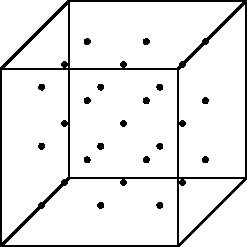
\includegraphics[width=0.25\textwidth]{Box_particles.pdf}
\caption{\small Schematic depiction of a box of size $\mathsf{R}$ including $N$ particle species.}
\label{fig:boxparticles}
\end{center}
\end{figure}
%%%%%%%%%%%
Given these state of affairs, one can easily estimate the number of possible configurations compatible with the above requirements. Indeed, if there are $N$ fundamental particle species, a simple thermodynamic analysis reveals that the macroscopic properties of the system would read as
%
\beq
\begin{aligned}
    E &= \mathfrak{c}_1\, N\, \mathsf{R}^{d-1}\, T^d\, ,\\
    S &= \mathfrak{c}_2\, N\, \left(\mathsf{R}\, T \right)^{d-1}\, ,
\end{aligned}
\label{eq:gasthermodynamics}
\eeq
%
where $T$ is the temperature of the system --- which we take to be much bigger than the masses of the particles involved, $S$ denotes its entropy and $\{ \mathfrak{c}_1, \mathfrak{c}_2\}$ are certain numerical constants that will not be important for our considerations here. Furthermore, upon solving for the temperature and imposing the restriction \eqref{eq:boundEnergyBH}, one obtains the following upper bound for the entropy inside the spherical region (in units where $G_N =1$)
%
\beq
\begin{aligned}
    S\, \leq\, \mathfrak{c}_3\, \left(N\, A^{d-1} \right)^{\frac{1}{d}}\, ,
\end{aligned}
\label{eq:entropyvsA}
\eeq
%
which only depends on the area of the $\mathbf{S}^{d-2}$ surface and the number of species. It is important to stress the fact that the bound \eqref{eq:entropyvsA} can be saturated precisely when the system is close to collapse into a black hole. 

Crucially, it has been argued that the maximum information content of any given spacetime region with dynamical gravity must be bounded from above by its surrounding area, namely
%
\beq
\begin{aligned}
    S\, \leq\, \frac{A}{4}\, .
\end{aligned}
\label{eq:entropybound}
\eeq
%
This has been conjectured to be a fundamental property of quantum-gravitational systems and is moreover formulated in terms of the \emph{holographic principle} \cite{tHooft:1993dmi,Susskind:1994vu,Bousso:1999xy, Bousso:1999cb}, which posits that the entropy bound \eqref{eq:entropybound} hinges on the total number of independent degrees of freedom in an underlying theory of quantum gravity. Notice that an area-law behaviour rather than the common volume growth in field theory is familiar from our experience with certain gravitational systems such as black holes, which indeed saturate  \eqref{eq:entropybound}. Moreover, if we assume the number of species $N$ to be small (say of $\mathcal{O}(1)$), then for spacetime regions which are large in Planck units, the entropy of the system satisfies the gravitational bound with room to spare, namely
%
\beq
\begin{aligned}
    S\, \lesssim\, A^{\frac{d-1}{d}}\, \ll\, \frac{A}{4}\, .
\end{aligned}
\eeq
%
On the other hand, precisely when the size of the $\mathbf{S}^{d-2}$ hypersurface becomes of order $\ell_d$, one finds a naive violation of the bound \eqref{eq:entropybound}, which tells us that this is the minimum length where semi-classical gravity makes sense, in accordance with our discussion in Section \ref{ss:basics}. Interestingly, if $N$ becomes instead very large, then a comparison between \eqref{eq:entropyvsA} and the maximum holographic entropy leads to the conclusion that the minimum length-scale that Einstein gravity can reliably describe grows with the number of species as follows (see also \cite{Vafa:2024fti})\footnote{\label{fnote:minentropyBH}Notice that this simple argument implies that the minimum holographic entropy in the presence of a large number of species grows like $S_{\rm min} \gtrsim N$.}
%
\beq
\begin{aligned}\label{eq:specieslength}
    \ell_{\rm sp} = \ell_d\, \left(\frac{N}{4\pi} \right)^{\frac{1}{d-2}}\, ,
\end{aligned}
\eeq
%
which in terms of energy cut-offs would read as
%
\beq
\begin{aligned}\label{species}
    \LSP = \frac{\Mpd}{N^{\frac{1}{d-2}}}\, .
\end{aligned}
\eeq
%
This energy scale is usually referred to as the \emph{species scale}, and was introduced (and further discussed) in the context of gravitational interactions in \cite{Han:2004wt,Arkani-Hamed:2005zuc, Distler:2005hi, Dimopoulos:2005ac, Dvali:2007hz, Dvali:2007wp, Dvali:2010vm}. Note that when the number of light species becomes parametrically large --- which happens e.g., when probing infinite distance limits in field space --- the separation between the Planck scale and the actual quantum gravity cut-off may be rendered parametric as well. 

Alternatively, one may argue for the existence of a species scale using black hole physics, by defining the latter as determining the smallest possible black hole in the theory, which we review now. The argument relies on the fact that black holes of size given by $\ell_{\rm sp}=\LSP^{-1}$ (thus much larger than the Planck length, $\ell_d$) have a lifetime --- due to Hawking radiation --- roughly of $\mathcal{O}(\ell_{\rm sp})$, and hence they should already probe the microscopic theory of gravity \cite{Dvali:2007hz, Dvali:2007wp}. That is, the smallest size for a semi-classical black hole is given by $\ell_{\rm sp}$ instead of $\ell_d$. To see this, let us consider the decay rate of a $d$-dimensional black hole of mass $\MBH$ into $N$ light species. This is computed to be \cite{Dvali:2007wp} 
%
\beq\label{eq:BHmassloss}
	\frac{d\MBH}{dt}\, \sim\, -N T_{\text{BH}}^2\, ,
\eeq
%
where $T_{\text{BH}}=R_{\text{BH}}^{-1} \sim \left( \Mpd^{d-2}\, \MBH^{-1}\right)^{\frac{1}{d-3}}$ denotes its Hawking temperature, which is assumed to be much larger than the masses of the individual particle states (see Section \ref{ss:Planck&string} for a more refined computation). From this, one can estimate the lifetime of the black hole by integrating \eqref{eq:BHmassloss} up to a temperature of order of the species cut-off, as follows
%
\beq
	\tau\ \sim\ \frac{1}{N} \int_0^{\Mpd ^{d-2}/\LSP^{d-3}} \text{d}\mu\ \left( \frac{\mu}{\Mpd^{d-2}}\right)^{\frac{2}{d-3}}\ \sim\  \ell_{\rm sp}\, ,
\eeq
%
where the upper limit corresponds to the mass associated to $T_{\text{BH}} = \LSP$, and in the last step we have used \eqref{species}. This strongly supports the idea that semi-classical, neutral, non-rotating black holes must be larger than $\LSP^{-1}$, which should therefore be identified as the quantum gravity cut-off. %Interestingly enough, as discussed in \cite{Dvali:2007hz}, one can also refine this non-perturbative computation to include the leading corrections to the species bound expression, which turn out to behave also as $\log N$ for large $N$, in agreement with our previous perturbative considerations. 

\subsection{Perturbative analysis}
\label{ss:perturbative}

%%%%%%%%%%%
\begin{figure}[htb]
\begin{center}
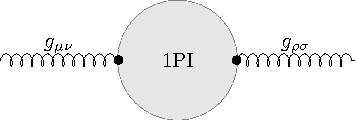
\includegraphics[width=0.5\textwidth]{1PI_graviton_2pt_function.pdf}
\caption{\small 1PI graviton self-energy. At one-loop order, matter fields contribute to the diagram as explained in the text, c.f. eqs. \eqref{eq:gravitonpropagator} and \eqref{eq:selfenergy}.}
\label{fig:1PIgraviton}
\end{center}
\end{figure}
%%%%%%%%%%%

The existence of an energy cut-off in gravity which is smaller than the Planck scale (in the presence of a large number of light degrees of freedom) can be motivated as well using a different class of arguments that are perturbative in nature. The idea hinges on studying the contribution of quantum corrections to the Einstein-Hilbert term in the Wilsonian effective action due to the interaction of gravity with $N$ particle species (see also \cite{Caron-Huot:2022ugt} for a related discussion in the context of S-matrix bootstrap). Strictly speaking, since gravity is non-renormalizable (c.f. Section \ref{ss:basics}), there is no sensible way to absorb the momentum dependence of loop corrections into a running coupling constant \cite{Anber:2011ut, Heidenreich:2017sim}. However, one can still estimate the scale at which amplitudes including loops become significant, thus breaking down the perturbative series. Including such loop corrections from the $N$ species minimally coupled to the gravitational field then results in a weakening of gravity by a factor of $1/N$ \cite{Donoghue:1994dn,Aydemir:2012nz,Anber:2011ut,Calmet:2017omb,Han:2004wt}. To see this, one can take the resummed one-loop propagator of the graviton in Lorentzian signature (for concreteness we consider a 4d flat background here although the computation can be easily extended to higher dimensions)
%
\beq \label{eq:gravitonpropagator}
	\i \Pi^{\mu \nu \rho \sigma}= \i \left(P^{\mu \rho} P^{\nu \sigma} + P^{\mu \sigma} P^{\nu \rho}-P^{\mu \nu} P^{\rho \sigma} \right)\, \pi(p^2)\ ,
\eeq
%
with $P^{\mu \nu}= \eta^{\mu \nu}-\frac{p^{\mu} p^{\nu}}{p^2}$ a projection operator onto polarization states transverse to $p^{\sigma}$ (i.e. it satisfies $P^{\rho}_{\sigma} P^{\sigma}_{\kappa}=P^{\rho}_{\kappa}$) and\footnote{Here $N$ is a weighted sum of light degrees of freedom. In four dimensions one has $N=N_s/3+N_f+4N_V$, with $N_s$ the number of real scalars, $N_f$ that of Weyl spinors and $N_V$ denotes the number of vectors \cite{Han:2004wt,Aydemir:2012nz}.}
%
\beq \label{eq:selfenergy}
	\pi^{-1}(p^2)=2p^2 \left( 1-\frac{N p^2}{120 \pi \Mpf^2}\, \log (-p^2/\mu^2) \right )\, .
\eeq
%
Therefore, one can now ask what is the momentum $p^2$ of the external graviton states for which the perturbative expansion breaks down, which happens precisely when the second term inside the parenthesis of \eqref{eq:selfenergy} becomes comparable to the first one, i.e. the tree-level contribution. Notice that in the one-loop propagator above there is an additional energy scale, $\mu$, which is related to the renormalization of certain quadratic terms in the curvature that typically appear at next order in the derivative expansion of the gravitational EFT \cite{Aydemir:2012nz}. Ignoring the logarithmic factor, one indeed recovers \eqref{species} up to $\mathcal{O}(1)$ coefficients from the above expression, signalling the energy scale where gravity presumably becomes strongly coupled.\footnote{See also Appendix A.2 in \cite{Heidenreich:2017sim} for a simple argument extending these perturbative considerations to higher-point functions derived from the on-shell graviton S-matrix.}

It is important to stress here the fact that there is actually nothing special about the previous perturbative argument, which clearly resembles other similar calculations of the wave-function renormalization of massless scalar fields or in (non-Abelian) gauge theories. There, depending on the number of colours and/or matter content, one can also encounter similar enhancement factors. The crucial difference in the context of gravitational theories is that \emph{(i)} gravity couples to everything that carries energy and momentum, in contrast to the scalar/gauge scenario where only `charged' particles contribute, and \emph{(ii)} the interaction itself is universal (at least in its minimal version) --- per the Equivalence Principle \cite{Wald:1984rg}, which is captured in the linearized lagrangian by a term of the form
%
\begin{equation}
\mathcal{L}_{\rm int} \supset \kappa_d \left( T^{\mu \nu} h_{\mu \nu}\right)\, ,
\end{equation}
%
where $h_{\mu \nu}(x)$ is the perturbation around the background metric $\bar{g}_{\mu \nu}$, c.f. eq. \eqref{eq:metricfluctuations}.

Oftentimes, when trying to compute explicitly what is the species cut-off associated to a certain spectrum of relatively light fields (or towers), one resorts to simple counting techniques that are related to the above perturbative calculation. In fact, what one does in practice is to compute both the number of species and the cut-off $\LSP$ at the same time in a self-consistent way, namely upon imposing $N$ to account for those degrees of freedom which lie below the species scale itself. Later on in Section \ref{ss:Planck&string}, we will provide explicit examples of this procedure. However, it is important to remark that the counting technique should only be taken as a book-keeping device yielding just an approximate answer which can actually differ from the exact result, especially when dealing with infinite towers of massive states.

\begin{comment}
However, they can be in principle included in the perturbative computation to calculate the corrections to the species scale. Thus, taking the renormalization scale $\mu$ to be fixed at or below $\Mpd$, one obtains the following implicit equation for $\LQG$
%
\beq 
	\Mpd^{d-2}\, \simeq\, N\, \LQG^{d-2}\, \log (\mu/\LQG)\, .
\eeq
%
This can be solved explicitly for $\LQG$ as follows
%
\beq 
	\LQG^{d-2} \simeq - (d-2) \frac{\Mpd^{d-2}}{N}\left\{ W_{-1} \left( -\frac{d-2}{N} \left[ \frac{\Mpd}{\mu} \right]^{d-2}\right)  \right\}^{-1}\, ,
\label{eq:speciesW-1}
\eeq
%
where $W_{-1}$ refers to the ($-1$)-branch of Lambert $W$ function.\footnote{\label{fn:Lambert} The Lambert $W$ function is defined as a solution to the equation
%
\beq
	\notag y\ e^y = x \iff y= W (x)\, .
\eeq
%
It has two real branches, namely  the principal branch, denoted  $W_0 (x)$ (defined for $x\geq 0$),  and the (-1)-branch, denoted $W_{-1}(x)$ (defined for $ -\frac{1}{e} \leq x < 0$). The asymptotic expansions that are relevant for this work take the form \cite{Lambert}
%
\beq
\label{eq:Wexpansion}
		\begin{split}
			&W_{0}(x\to \infty)\, =\, \log (x)-\log (\log(x))+\ldots\\
			&W_{-1}(x\to 0^-)\, = \, \log (-x)-\log (-\log(-x))+\ldots
		\end{split}
\eeq
%
} Given the asymptotic properties of $W_{-1}(x)$ at $x \to 0^{-}$ (c.f. eq. \eqref{eq:Wexpansion}), such solution for the species scale seems to approach zero in Planck units when $N \to \infty$, as it should be, and can be interpreted as correcting the $N$ dependence in eq. \eqref{species} by sending $N \to N\, \left|W_{-1} \left ( - \frac{d-2}{N}\right)\right|$, which is indeed a logarithmic correction roughly of the form $N\to N\, \log N$. This then justifies  the definition \eqref{species} up to logarithmic corrections. Such corrections both to the species scale and  to the number of species, $N$, may play a crucial role in some situations (e.g. when calculating the species scale for a tower of stringy states), in which case we will include them, whereas they can be safely ignored in some others, where they do not seem to change the results qualitatively. In the following, we will explicitly display them whenever relevant or necessary.
\end{comment}

\section{The species scale in quantum gravity}
\label{s:speciesscale} 

The main goal of this thesis is to fully grasp the role and provide a proper definition of the relevant energy cut-off in gravity, understood as the scale at which quantum gravitational effects can no longer be neglected and local effective field theory breaks down. We have already introduced in Section \ref{s:speciesmotivation} some particular energy scale which depends on the number of light degrees of freedom existing in our theory, which we dub the species scale $\LSP$ (c.f. eq. \eqref{species}). Such cut-off was motivated using various different arguments, ranging from the perturbative physics of the massless graviton in the presence of a large amount of degrees of freedom, to a non-perturbative black hole/holography analysis which imposes some minimal length-scale in gravity. In this section, we want to provide a unifying picture from which all these considerations would naturally follow, as well as discuss the value of $\LSP$ in realistic string theory/quantum gravity vacua.

Therefore, the precise statement would be, following the logic of Section \ref{ss:basics}, that the lagrangian density of any gravitational effective field theory is organized according to the energy expansion
%
\beq
\mathcal{L}_{\mathrm{EFT}}\, =\, \sqrt{-g}\, \dfrac{1}{2\kappa_d^2}\left(\mathcal{R} + \sum_{n \geq 2} \frac{\mathsf{O}_n (\mathcal{R})}{\LSP^{n-2}}\right)\, +\, \ldots\, ,
\label{eq:gravEFTexpansion}
\eeq
%
where we have substituted $\LQG = \LSP$ in eq. \eqref{eq:gravEFT}, such that the species scale controls/suppresses \emph{generic} local gravitational corrections. The ellipsis in \eqref{eq:gravEFTexpansion} indicates any other couplings and matter fields present in the effective field theory. From this perspective it becomes clear how the previous (non-)perturbative arguments arise. In the former case, when computing any scattering amplitude involving graviton states in the external legs, as soon as we consider energies close to $\LSP$ we find that an infinite number of higher-curvature and higher-dimensional corrections become relevant, spoiling any naive analysis involving just the two-derivative term. On the other hand, for black holes which are small enough so as to probe the cut-off scale, one typically finds curvatures of order $\ell_{\rm sp}^{-2}$, thus inducing important corrections to e.g., the Bekenstein-Hawking entropy obtained solely from the Einstein-Hilbert action \cite{Sen:2005wa}.

Let us also mention that, in principle, different kinds of higher-dimensional operators can arise in a given gravitational theory, and not all of them need to be a priori suppressed by a single ultra-violet scale \cite{Donoghue:1995cz}. For instance, one may get threshold contributions in the Wilsonian effective action once we integrate out some massive particle(s), and which can ultimately dominate over the suppression given by the quantum gravity cut-off in \eqref{eq:gravEFTexpansion}. Still, this should not be regarded as a drawback in the identification of the species scale from higher-curvature operators, since these couplings naturally depend on the energy scale at which they are measured. Hence, a more accurate statement would be that the suppression of generic higher-curvature operators in the gravitational EFT is controlled by $\LSP$ when measured at energies close to the cut-off itself, see Chapter \ref{ch:Higherdimops} for details on this point.
	

\subsection{Why you get old}
\label{ss:Planck&string}

The fact that the Planck scale does not actually provide for the ultra-violet cut-off in effective field theories consistent with quantum gravity is strongly supported by the string theory landscape. There, the lower dimensional Planck mass usually depends on the details of the string theory embedding, such as the fundamental vibrating string that we start with as well as the size of the compact internal dimensions. In this section we analyze the behaviour of the species cut-off \eqref{species} in realistic string theory constructions. Along the way, we will realize that it matches the expectations both in Kaluza-Klein theories of gravity and string theory, therefore providing for a unifying concept that defines the maximum regime of validity of any given EFT weakly coupled to Einstein gravity, regardless of its UV completion. Our strategy here will consist in focusing on asymptotic regions within field space, where the species counting proceeds in an easier way thanks to the weak coupling behaviour exhibited by the theory, which helps in determining both its massive spectrum as well as in organizing the EFT expansion according to eq. \eqref{eq:gravEFTexpansion}. Indeed, in these extreme regimes the Distance Conjecture \cite{Ooguri:2006in} predicts the appearance of infinite towers of exponentially light particles, which become asymptotically stable resonances of the theory. Moreover, per the Emergent String Conjecture \cite{Lee:2019wij}, one only expects two such different scenarios to emerge: either the theory decompactifies to a higher-dimensional one, or one reaches a weak coupling limit for an emergent critical string (not necessarily the original one). The relevant towers of nearly massless states thus become Kaluza-Klein replica --- with spin $s \leq 2$, or rather the excitation modes of a fundamental string, which include higher-spin particles as well. Hence, in what follows we will consider both scenarios in turn, analyzing the behaviour of the species scale in the presence of the aforementioned light towers.
	
\subsubsection{Species scale from Kaluza-Klein towers}\label{sss:KKtowersspecies}
	
Consider a $d$-dimensional EFT describing the physics of $N_0$ massless/light modes, weakly coupled to Einstein gravity. In particular, let us assume this theory as coming from the dimensional reduction of some $(d+k)$-dimensional gravitational EFT. For simplicity, we take the higher-dimensional theory to be compactified on an isotropic and rectangular torus $\mathbf{T}^k$, of radius $R$ measured in $(d+k)$-dimensional Planck units. That is, in our conventions $R$ is dimensionless and the physical size of the $k$-torus is given by $\left( 2\pi R\, \ell_{d+k}\right)^k$, where $\ell_{d+k}$ denotes the higher-dimensional Planck length. For this set-up, the Planck scales of the lower and higher dimensional theories are related as follows
%
\beq
	\Mpd^{d-2}\, =\, M_{\text{Pl};\, d+k}^{d-2}\, (2\pi R)^k\, ,
	\label{eq:Planckscales}
\eeq
%
whereas the mass scale of the $k$ corresponding  KK towers reads\footnote{Each of these towers is indeed associated to internal momentum of the higher dimensional fields along the $k$ different directions in the compactification space. Notice that particles with multiple KK charges do exist, and thus the degeneracy of states grows roughly as the product of the maximum excitation numbers, see Section \ref{ss:MultipleTowers}.}
%
\beq\label{eq:KKmass}
	\MKK\, =\, \dfrac{M_{\text{Pl};\, d+k}}{R}\, .
\eeq
%
If we approach now the large volume point, namely the limit $R\to \infty$, the Kaluza-Klein towers become light in an exponential fashion with the proper field distance, as predicted by the Distance Conjecture (see Section \ref{s:SDC}). With this, we can then determine the species scale associated to such a dense tower of light states. We will use perturbative and non-perturbative arguments to compute $\LSP$ in the present case, leading both ultimately to the same quantitative answer.

\subsubsection*{Determining $\LSP$ via species counting}

Let us assume that every light mode in the $d$-dimensional EFT has its own KK replicas. Equivalently, we think of the lower dimensional theory to be propagating as well in the higher-dimensional bulk, in contrast to when e.g., it is localized on a brane. As a consequence, one can estimate the total number of states $N$ below the UV cut-off as follows
%
\beq
	N\, \simeq\, N_0 \left( \frac{\LSP}{\MKK} \right)^{k}\, .
	\label{eq:numberKKmodes}
\eeq
%
Combining now eqs. \eqref{species} and \eqref{eq:Planckscales}, we arrive at the following species cut-off
%
\beq\label{eq:speciesscaleKK}
	\LSP^{d+k-2}\, \simeq\, \frac{\Mpd^{d-2}\, \MKK^k}{N_0}\, \simeq\, \frac{M_{\text{Pl};\, d+k}^{d+k-2}}{N_0}\, .
\eeq
%
Notice that what we obtain is precisely the species scale associated to the higher dimensional theory, including the $N_0$ fields already present there. That is, the species scale of the $d$-dimensional EFT provides the right cut-off that one would expect to find in the UV theory, namely the $(d+k)$-dimensional $\LSP$.\footnote{Notice that this simple argument makes manifest the fact that the definition/concept of species scale is consistent (or preserved) under dimensional reduction.} %Let us emphasize the important role played here by the $N_0$ light species which are already present in the higher dimensional theory, and thus correct its QG cut-off from the naive $(d+k)$-dimensional Planck mass to the corresponding species scale. 
Hence, the intuitive result that the higher-dimensional Planck mass captures the quantum gravity cut-off is thus recovered when $N_0=\mathcal{O}(1)$.

\subsubsection*{Determining $\LSP$ via black holes}

One can arrive at essentially the same result for $\LSP$ upon studying black holes of minimal size instead (c.f. Section \ref{ss:nonperturbative}). This allows us to give more evidence for the picture advocated in this chapter. In fact, we can argue for the relation \eqref{eq:speciesscaleKK} in two different ways: \emph{(i)} by determining the size of the black hole whose microstates saturate the minimum holographic entropy $S_{\rm min} \gtrsim N$ (see \cite{Blumenhagen:2023yws, Calderon-Infante:2023uhz} for similar considerations), and \emph{(ii)} upon finding those black holes whose typical evaporation time is already of the order of their size \cite{BHdecaynotes}. 

Let us consider first the microscopic entropy associated to the smallest possible neutral black hole that can be constructed in the theory, namely one with radius $\mathsf{R}= \ell_{\rm sp}$. Its associated mass would read as
%
\beq\label{eq:massminimalBH}
	M_{\rm BH,\, min} = \frac{(d-2) \pi^{\frac{d-3}{2}}}{8\, G_N\, \Gamma (\frac{d-1}{2})}\, \ell_{\rm sp}^{d-3}\, .
\eeq
%
We can now estimate the contribution of \emph{uncharged} Kaluza-Klein modes to the Bekenstein-Hawking entropy of such minimal black holes by finding the total number of microstates compatible with the constraint \eqref{eq:massminimalBH}. For simplicity, we work in the following with a KK spectrum corresponding to a single decompactifying dimension of topology $\mathbf{S}^1/\mathbb{Z}_2$. In that case, the maximum occupation number in the tower that can contribute to the BH entropy is
%
\beq
	\mathsf{N}= \frac{M_{\rm BH,\, min}}{\MKK}\, ,
\eeq
%
whilst the total number of microstates comprised by combinations of Kaluza-Klein modes is given by the number of partitions of $\mathsf{N}$. In the decompactification limit, where this quantity becomes large, we can approximate the total amount of microscopic configurations as follows
%
\beq
	\Omega = p(\mathsf{N}) \sim \frac{1}{4\, \sqrt{3}\, \mathsf{N}} \exp \left( \sqrt{\frac{2\, \pi^2\, \mathsf{N}}{3}} \right)\, , \qquad \text{for}\ \ \mathsf{N} \gg 1\, ,
\eeq
%
where we used the Hardy-Ramanujan formula above. Therefore, the entropy associated to a black hole of mass $M_{\rm BH,\, min}$ would be given by 
%
\begin{align}\label{eq:statentropyKK}
	S_{\rm BH,\, min} := \log \Omega = \sqrt{\frac{2\, \pi^2\, \mathsf{N}}{3}}\, +\, \mathcal{O} \left(\log \mathsf{N}\right)\, \sim\, \left( \frac{\ell_{\rm sp}^{d-3} \Mpd^{d-2}}{\MKK}\right)^{1/2}\, \sim\, N\, ,
\end{align}
%
where in the last step we made use of the definition of $\LSP$ as well as $N= \LSP/\MKK$. This is in precise agreement (up to numerical factors) with the minimum holographic entropy in the presence of $N$ Kaluza-Klein species, such that we conclude that $\ell_{\rm sp}$ --- as defined in \eqref{eq:specieslength} --- correctly determines the minimum black hole size. Equivalently, one may ask for the point where the statistical entropy \eqref{eq:statentropyKK} equals that of a black hole of mass $M_{\rm BH}$, which happens when 
%
\begin{align}\label{eq:transitionpointBHtoKK}
	M_{\rm BH}^{d-1}\, \sim\, \frac{\Mpd^{2(d-2)}}{m_{\rm KK}^{d-3}} \Longrightarrow R_{\rm BH}\, \sim\, m_{\rm KK}^{\frac{-1}{d-1}}\, \Mpd^{\frac{2-d}{d-1}}\, ,
\end{align}
%
i.e. precisely when the black hole has a size of order of the species cut-off $\ell_{\rm sp}$, c.f. eq. \eqref{eq:speciesscaleKK}.

On the other hand, it is possible to argue for \eqref{eq:massminimalBH} as capturing the minimal semi-classical black hole mass by studying its typical evaporation time (via Hawking radiation) in the presence of the KK tower. Indeed, consider the generic case where the internal space is given by some Ricci-flat $k$-dimensional compact manifold $\mathcal{X}_k$, with a mass spectrum of the form\footnote{The relation \eqref{eq:spectrumLaplaciannmfd} follows essentially from the WKB approximation, which can be understood here as simply saying that for highly excited modes, the spectrum of the laplacian behaves roughly as in e.g., a toroidal manifold with the same number of dimensions.}
%
\begin{align}\label{eq:spectrumLaplaciannmfd}
	m_n\, \sim\, n\, \MKK\, , \qquad \text{for}\ \ n \gg 1\, .
\end{align}
%
Thus, to compute the evaporation time one needs to solve the following differential equation
%
\begin{equation}\label{eq: deg t}
    \frac{d M_{\rm BH}}{d t}\, \sim\, - T_{\rm BH}^2\sum_{n=0}^{\infty}d_{n}(\mathcal{X}_k)\left(e^{-\frac{\MKK}{T_{\rm BH}}}\right)^{n}\,,
\end{equation}
%
where $d_n(\mathcal{X}_k)$ denotes the degeneracy of each mass eigenmode $m_n$ in the tower (i.e. the number different states with $m=m_n$) and we have included an additional Boltzmann suppression factor $e^{-\frac{m_n}{T_{\rm BH}}}$ with respect to \eqref{eq:BHmassloss}. Moreover, using Weyl's asymptotic formula
%
\begin{equation}
    N(\lambda)\, \sim\, \lambda^{k/2}\, \text{vol} \left( \mathcal{X}_k\right),\qquad \text{for}\ \ \lambda\to\infty\, .
\end{equation}
%
which accounts for the number of accumulated eigenvalues $\lambda$ of the Laplace-Beltrami operator acting on functions defined over $\mathcal{X}_k$, we can readily estimate the degeneracy to be\footnote{Even though \eqref{eq:asymptoticdegeneracyKK} gives only an approximation for large KK masses, in certain cases it may be possible to determine $d_n(\mathcal{X}_k)$ exactly. For instance, if $\mathcal{X}_k$ is a $k$-sphere, one finds (c.f. eq. \eqref{eq:deg10-dsphere})
%
\begin{equation}\label{eq:asymptoticdegeneracyKK}
    \notag d_n(\mathbf{S}^k)=\frac{(n+k-2)!(2n+k-1)}{n!(k-1)!}\, \sim\, \frac{2}{(k-1)!}n^{k-1}\, .
\end{equation}
}
%
\begin{equation}
    d_n(\mathcal{X}_k) = N(m_n)-N(m_{n-1})\, \sim\, n^{k-1}\, .
\end{equation}
%
With this in mind, we can then go back to \eqref{eq: deg t} and rewrite it as follows
%
\begin{align}
     \frac{d M_{\rm BH}}{d t}\, &\sim\, -T_{\rm BH}^2\sum_{n=0}^{\infty}n^{k-1}\, e^{-n\, \frac{\MKK}{T_{\rm BH}}}\, =\, -T_{\rm BH}^2\, \left( -\frac{d}{dx}\right)^{k-1} \frac{1}{1-e^{-x}}\bigg\rvert_{x=\frac{\MKK}{T_{\rm BH}}} \notag\\
     &=-T_{\rm BH}^2\, (k-1)!\,  \left(\frac{T_{\rm BH}}{\MKK}\right)^k\, +\, \mathcal{O} \left( \left(\frac{\MKK}{T_{\rm BH}}\right)^0 \right)\, ,
\end{align}
%
where we have first resummed the series in terms of an auxiliary variable $x=\frac{\MKK}{T_{\rm BH}}$ and subsequently expanded the result assuming $T_{\rm BH} \gg \MKK$ all along the evaporation process. Hence, integrating the previous differential equation yields 
%
\begin{align}\label{eq: tau int}
    \tau&\sim \MKK^k\int_0^{M_{\rm BH,\, min}}T_{\rm BH}(\mu)^{-k-2}\dd \mu\, \sim\, \MKK^k\, M_{{\rm Pl;}\, d}^{-\frac{(k+2)(d-2)}{d-3}}\int_0^{M_{\rm BH,\, min}}\mu^{\frac{k+2}{d-3}}\dd \mu\notag\\
    &\simeq\, \MKK^k\, M_{{\rm Pl;}\, d}^{-\frac{(k+2)(d-2)}{d-3}} M_{\rm BH,\, min}^{\frac{d+k-1}{d-3}}\, \sim\, \MKK^k\, M_{{\rm Pl;}\, d}^{d-2}\, \LSP^{-d-k+1}\,,
\end{align}
%
where in the last step we have substituted \eqref{eq:massminimalBH}. Finally, upon inserting \eqref{eq:numberKKmodes} as well as the definition of the species scale we find that
%
\begin{equation}
    \tau\, \sim\, \ell_{\rm sp}\, ,
\end{equation}
%
in agreement with our previous arguments.
	
%Before turning into the computation of the species scale for stringy towers, let us remark a couple of key properties of general KK-like towers that make them qualitatively different from stringy ones, and play a crucial role in the computation of the species scale. First, there is the fact that there can be multiple KK-towers, with different charges and (possibly) different mass scales, which can lie below the species cut-off. We elaborate on this in section \ref{ss:MultipleTowers} but it is worth remarking it here as opposed to the case of stringy towers, for which only one critical string can become light at the same time. Second, the structure of KK towers is such that the degeneration of states in each step of the tower (i.e. for a given mass) grows at most polinomially, in contrast to the well-known exponential degeneration that appears for the high excitation levels of a string \cite{Green:2012oqa}.
	
\subsubsection{Species scale from string towers}\label{sss:stringtowersspecies}
	
We turn now to the case in which the tower of states is provided by the excitation modes of a fundamental critical string that becomes asymptotically tensionless. Here the situation is dramatically different, since as it is well-known the associated higher-spin towers present a much denser spectrum than their Kaluza-Klein counterparts. The reason for this is twofold: first, in flat backgrounds, the string oscillators are characterized by having a mass given roughly by the Regge excitation pattern 
%
\beq
	m_n^2\,=\, 8\pi T_s \left(n-1\right)\, ,
\label{eq:stringmasses}
\eeq
%
where $T_s=2 \pi m_s^2$ denotes the string tension and $n \in \mathbb{N}$ refers to the excitation/oscillator level of the critical string. Second, one has to take into account the high level density of modes, $d_n$, associated to the very massive excited states. In fact, to leading order, for large $n$  this degeneracy behaves in an exponential fashion \cite{Green:2012oqa}
%
\begin{align}\label{eq:exactleveldensitystrings}
     d_n & \sim\, n^{-11/2}\, \e^{4\pi \sqrt{2n}}\, , \qquad \qquad \ \text{for Type II strings}\, , \notag\\
     d_n\, &\sim\, n^{-11/2}\, e^{2 \pi (2+\sqrt{2}) \sqrt{n}}\, , \qquad \text{for Heterotic strings}\, .
\end{align}
%
With these ingredients we can then study both perturbatively and non-perturbatively the behaviour of the species scale in the presence of string oscillator towers. As we will explicitly demonstrate, both approaches lead to the same \emph{qualitative} answer, even though they might differ quantitatively due to the validity of the corresponding computational methods.

\subsubsection*{Determining $\LSP$ via species counting}
	
We proceed first via the usual state counting algorithm, which is based on the perturbative argument provided in Section \ref{ss:perturbative}. Let us stress that since that discussion was phrased using purely field-theoretic considerations, a direct application of these ideas to an infinite set of particles containing higher-spin states is strictly speaking not suitable anymore. However, this crude prescription will provide us with some potential candidate for $\LSP$ that is qualitatively similar to the exact one, see below. Moreover, the route followed in this section will also be amenable to certain string theory applications discussed in Part \ref{part:StringTheoryTests} of this thesis. Hence, it is instructive to perform the exercise at this point.

In order to be as general as possible, let us consider some $d$-dimensional EFT where we take the weak coupling limit corresponding to some fundamental string. Consequently, the associated oscillator modes become asymptotically massless when measured in Planck units, since their masses are proportional to 
%
\beq\label{eq:ddimdilaton}
	\frac{m_s}{\Mpd} = (4 \pi)^{2-d}\, g_d^{2/d-2} \to 0\, ,\qquad \text{as}\ \ g_d \to 0\, ,
\eeq
%
where $g_d$ denotes the $d$-dimensional string coupling. To compute $\LSP$ we first need to know what is the maximum excitation level $\Ns$ whose mass lies at or below the species cut-off. Subsequently, we need to count the number of accumulated string modes up to such $\Ns$, which we denote by $N$ in the following. The species scale thus fulfills
%
\beq
\label{eq:speciescale}
	\LSP^{d-2}\, \simeq\, \frac{\Mpd^{d-2}}{N}\, \simeq\, \Ns^{\frac{d-2}{2}}\, \Ms^{d-2}\, .
\eeq
%
Rearranging the above equation we arrive at
%
\beq
\label{eq:Ns}
	\Ns^{\frac{d-2}{2}} \sum_{n=1}^{\Ns} d_n \, \simeq\, \left ( \frac{\Mpd}{\Ms}\right )^{d-2}\, ,
\eeq
%
where we have substituted $N =\sum_{n=1}^{\Ns} d_n$ in terms of the sum over the density levels of physical states in the string tower. Next, one needs to substitute the explicit form \eqref{eq:exactleveldensitystrings} of the degeneracy of the oscillators, and then solve for $\Ns$. In what follows, we will approximate $d_n$ by the simplified quantity
%
\beq
	d_n\, \sim\, e^{ \sqrt{n}}\, ,
	\label{eq:leveldensity}
\eeq
%
since this is enough for our purposes here and already captures the key asymptotic behaviour of $\LSP$.\footnote{See Appendix A of \cite{Castellano:2022bvr} for a more accurate computation in all the relevant string theories considered in this thesis.} Upon doing so, one finds 
%
\beq
	\left ( \dfrac{ \Mpd}{\Ms}\right )^{d-2}\, \simeq\, \Ns^{\frac{d-2}{2}} \sum_{n=1}^{\Ns} e^{\sqrt{n}} \, \sim\, 2\, \Ns^{\frac{d-1}{2}} e^{\sqrt{\Ns}}\, ,
\label{eq:maxstringlevel}
\eeq
%
where we have retained just the leading order term in the sum, which is justified in the limit where $\Ns \to \infty$. From this, we can obtain an explicit expression for $\Ns$ that reads
%
\beq
	\sqrt{\Ns}\, \sim\, (d-1)\, W_0 \left( \dfrac{1}{(d-1)\, 2^{\frac{1}{d-1}} } \left[ \dfrac{\Mpd}{\Ms} \right]^{\frac{d-2}{d-1}} \right)\, ,
\eeq
%
where $W_0$ refers to the principal branch of Lambert $W$ function.\footnote{\label{fn:Lambert} The Lambert $W$ function is defined as a solution to the equation
%
\beq
	\notag y\ e^y = x \iff y= W (x)\, .
\eeq
%
It has two real branches, namely  the principal branch, denoted  $W_0 (x)$ (defined for $x\geq 0$),  and the (-1)-branch, denoted $W_{-1}(x)$ (defined for $ -\frac{1}{e} \leq x < 0$). The asymptotic expansions that are relevant for this work take the form \cite{Lambert}
%
\beq
\label{eq:Wexpansion}
		\begin{split}
			&W_{0}(x\to \infty)\, =\, \log (x)-\log (\log(x))+\ldots\, ,\\
			&W_{-1}(x\to 0^-)\, = \, \log (-x)-\log (-\log(-x))+\ldots\, .
		\end{split}
\eeq
%
}
Crucially, the above equation reveals that the maximum excitation level of the string that falls below the cut-off scale diverges when $\Ms/\Mpd \to 0$, thereby confirming the approximations taken so far. Indeed, upon using the relevant expansion of the $W$-function from eq. \eqref{eq:Wexpansion}, such divergence can be seen to behave essentially in a logarithmic fashion, i.e.
%
\beq
	\sqrt{\Ns}\, \sim\, (d-2)\, \log \left(\dfrac{\Mpd}{\Ms}\right) + \mathcal{O}\left(\log \left( \log (\Mpd/\Ms) \right) \right)\, .
\eeq
%
This means that, according to this prescription, the species scale for a critical emergent string in $d$ spacetime dimensions would behave as  
%
\beq\label{eq:speciesforstringspert}
	\frac{\LSP}{\Mpd}\, \simeq\, \sqrt{\Ns}\, \frac{\Ms}{\Mpd}\, \sim\,  (d-2)\,  \dfrac{\Ms}{\Mpd}\  \log \left(\dfrac{\Mpd}{\Ms}\right)\, ,
\eeq
%
thus confirming our expectations that the quantum gravity cut-off should be given in this case by the string scale itself. Nonetheless, there seems to be important logarithmic corrections in \eqref{eq:speciesforstringspert} which are crucial in order to make sense of the state counting between $\LSP$ and $\Ms$, since they encode the asymptotic behaviour of $\Ns$. As we argue in what follows, however, we believe these additional factors to be unphysical as well as an artifact of using the field theoretic approach for a higher-spin tower.

\subsubsection*{Determining $\LSP$ via black holes}

We study now the same question from the perspective of black hole physics, namely we want to know what is the minimum size for a semi-classical black hole in the presence of a nearly tensionless fundamental string. Following the same logic as in the Kaluza-Klein scenario, we can solve the problem using two different approaches.

First, we want to find the transition point where the minimum holographic entropy is attained. Taking advantage of what we learned in the previous case, we can easily 
estimate this upon determining the mass (equivalently the radius) of the black hole where its entropy can be completely accounted for by the string oscillator modes \cite{Susskind:1993ws}. Let us thus confront both entropy functions. On the one hand, the entropy of a free string is proportional to its length \cite{Green:2012oqa} 
%
\beq
	S_{\rm string}\, \sim\, \frac{L}{\ell_s}\, \sim\, \frac{M_{\rm BH,\, min}}{m_s}\, ,
\eeq
%
whilst that of a (minimal) black hole reads as follows
%
\beq
	S_{\rm BH}\, \sim\, \left( R_{\rm BH,\, min}\, \Mpd \right)^{d-2}\, \sim\, \left(\frac{M_{\rm BH,\, min}}{\Mpd} \right)^{d-2}\, .
\eeq
%
Hence, by comparison between the two, we find
%
\begin{align}
	M_{\rm BH,\, min}\, \sim\, \frac{\Mpd^{d-2}}{m_s^{d-3}} \Longrightarrow R_{\rm BH,\, min}\, \sim\, \ell_s\, ,
\end{align}
%
namely the minimum black hole size is precisely of order of the string length. Stated differently, we reach the conclusion that $\LSP \simeq m_s$. Note that the previous analysis is actually rather crude, essentially because we ignored the self-gravitating effects of the string when comparing both behaviours.\footnote{In a sense, we were entitled to do so since by assumption we consider a regime of weak string coupling.} It turns out, however, that one can do slightly better and properly take into account these effects. This was done in \cite{Horowitz:1996nw,Horowitz:1997jc}, which ultimately led to the black hole-string correspondence, where it is claimed that in fact a typical uncharged black hole undergoes a transition to a highly excited and long (but compact) string precisely when it reaches a size of the order of $\ell_s$. (See also \cite{Chen:2021dsw} for a recent analysis of the black hole-string transition in Heterotic and Type II string theories.)

On the other hand, one may also argue for $\LSP \simeq m_s$ by studying the typical decay time of a black hole of stringy size. Indeed, the Hawking evaporation process in the presence of the string oscillator modes would read as
%
\begin{equation}\label{eq:BHtostringdecay}
    \frac{d M_{\rm BH}}{d t}\, \sim\, - T_{\rm BH}^2\sum_{n=1}^{\infty}n^{-\frac{11}{2}}\, \e^{\left(\beta_{\rm H}-\beta_{\rm BH}\right)\, m_n}\, ,
\end{equation}
%
where $\beta_{\rm BH} = 1/T_{\rm BH}$ and $\beta_{\rm H}$ denotes the inverse Hagedorn temperature of the corresponding critical string (which is thus proportional to the string length $\ell_s$, c.f. eq. \eqref{eq:exactleveldensitystrings}). Therefore, it is easy to check that when $T_{\rm BH} \ll T_{\rm H}$ (equivalently $\beta_{\rm BH} \gg \beta_{\rm H}$) one obtains
%
\begin{equation}
    \tau\, \sim\, \frac{e^{\frac{T_{\rm BH}}{T_{\rm H}}}}{T_{\rm BH}}\, \left( \frac{\Mpd}{T_{\rm H}}\right)^{d-2} \gg T_{\rm BH}^{-1}\, \sim\, R_{\rm BH}\, ,
\end{equation}
%
whereas if $T_{\rm BH} > T_{\rm H}$ the calculation \eqref{eq:BHtostringdecay} breaks down completely since at the Hagedorn point the thermal ensemble should stop being well-defined, even at large distances from the black hole. In fact, precisely when $\beta_{\rm BH} \gtrsim \beta_{\rm H}$ (with $\beta_{\rm BH}-\beta_{\rm H} \ll \ell_s$) it is the Horowitz-Polchinski saddle the one that dominates the dynamics of the system \cite{Horowitz:1997jc}.


\subsection{An algorithmic procedure in the presence of multiple towers}
\label{ss:MultipleTowers}

To end this section, let us address the more general scenario in which several towers with different charges and in principle distinct spectra are present. As we will discuss in later parts of this thesis, the following analysis is especially relevant in the context of string theory, since it is typically the case that not just one but actually several towers become light when probing asymptotic regions in field space. In particular, one could imagine a situation where as we approach an infinite distance point in moduli space, multiple towers get asymptotically massless and lie below the species cut-off, such that each one of them should contribute a priori to its computation --- since they all couple to the gravitational field. Given this state of affairs, one can think of two qualitatively different situations that may arise, depending on whether or not the towers form bound states between each other. We discuss each of them in turn in what follows.
	
\subsubsection*{Case I: Additive species}

 Let us first consider a set-up in which there is no mixing between the towers. This happens e.g., when we have two (infinite) sets of particles that couple to different fields and such that no states with both charges are present in the spectrum (of quasi-stable modes). In this case, the total number of species below the quantum gravity cut-off is given by $N_{\mathrm{tot}}= \sum_i N_i$, where $N_i$ is the number of states associated to the $i$-th tower. The species scale, as defined by eq. \eqref{species}, should then be computed by including all light particles arising from every tower. However, since the number of species --- below some fixed energy scale $\Lambda_{\rm UV}$ --- of any given set of light states diverges in the asymptotic limit, $N_{\mathrm{tot}}$ will be dominated essentially by just one of the towers (unless all $N_i$ scale in the same way with respect to the relevant moduli, in which case the following calculation would simply be modified by $\mathcal{O}(1)$ factors). In practice, we can calculate the would-be cut-off associated to each tower separately. Thus, consider a set of states with mass spectrum given by
%
\begin{equation}
\label{eq:Mni}
		m_{n,\, i}\, =\, n^{1/p_i}\ \Mti\, .
\end{equation}
%
Here, the parameter $p \in \mathbb{R}$ characterizes the spacing between different steps within the tower (of constant degeneracy), or equivalently it can be regarded as counting the number of towers with identical mass gap. (For instance, a standard Kaluza-Klein tower associated to a circular extra dimension has $p=1$.) In practical terms, however, it should be seen just as a book-keeping device which is useful when solving counting exercises as in the present case.\footnote{See \cite{Casas:2024ttx} for a recent example of a truly $p=2$ tower of particles.} We can then compute the species scale as follows
%
\begin{equation}\label{eq:speciesscaleithtower}
		\LSP{}_{,\, i}\, \simeq\, N_i^{1/p_i}\Mti\, \simeq\, \dfrac{\Mpd}{N_i^{\frac{1}{d-2}}}\, .
\end{equation}
%
The physical value for $\LSP$ would be given by the minimum out of the set $\{ \LSP{}_{,\, i} \}$, since it is dominated by the states corresponding to the tower with the lightest mass scale. For concreteness, let us label the leading tower by the index 1, characterized by the density parameter $p_1$ and mass gap $\frac{m_{\text{tow,}\, 1}}{\Mpd} \sim t^{-a_1}$, which goes to zero as we take some modulus $t$ to infinity. For all the remaining towers, we consider $\frac{\Mti}{\Mpd} \sim t^{-a_i}$. Since the set of light states is dominated by the first tower alone, we have $N_{\text{tot}}=N_1+\ldots\, \sim\, N_1$, and
%
\begin{equation}\label{eq:speciesadditive}
		N_1\, \sim\, t^{\frac{a_1 p_1(d-2)}{ d-2+p_1}}\, , \qquad  \LSP\, \sim\, \Mpd\, t^{-\frac{ a_1 p_1}{d-2+ p_1}}\, .
\end{equation}
%
To check the consistency of this picture, we can recalculate the number of states associated to the subleading towers --- i.e. the ones with $i\geq 2$ --- that lie below the $\LSP$ just determined. These read
%
\begin{equation}
		\tilde{N}_i\, \sim\, t^{\frac{(d-2) a_i p_i+ p_1 p_i (a_i - a_1)}{d-2+p_1}}\, ,
\end{equation}
%
and we find $\tilde{N}_i \ll N_i$, as expected. Note that this expression contains negative contributions in the exponent, corresponding to the case where a tower is still too heavy to provide any mode below $\LSP$.% as well as the case where an asymptotically infinite number of them are present.
	
Let us remark also that a stringy tower would correspond in this language to having $p \to \infty$.\footnote{To be precise, one would need to include the exponential degeneracy together with $p=2$, as we did in the previous section. Nonetheless, for the case at hand most of the calculations yield the correct result if we model such high degeneracy by just taking the limit $p \to \infty$. } It is thus clear that such a spectrum would completely dominate any set-up in which the string oscillators have to be taken into account, thus recovering the expected result $\LSP \sim m_s$ (see Section \ref{sss:stringtowersspecies} for details).
	
	
\subsubsection*{Case II: Multiplicative species}
Second, we consider the scenario in which the different towers are such that states with mixed charges can be present. This is the case that is actually relevant in most set-ups. It is realized by e.g., several KK towers since we can have states with non-vanishing momentum along various internal directions at the same time; or even in the presence of a fundamental string and Kaluza-Klein modes. In this case, the total number of species is not just additive, but rather multiplicative, i.e. $N_{\text{tot}}\simeq \prod_i N_i$. Thus, let us assume that we have $k \in \mathbb{N}$ generating towers of (asymptotically) light particles behaving again like \eqref{eq:Mni}, such that states with more than one non-vanishing occupation number appear in the spectrum, with a mass formula of the general form
%
\begin{equation}\label{eq:massmixedsprectra}
		m_{n_1\,  \ldots  n_k}^2\, =\, \sum_{i=1}^k n_i^{2 / p_i} \Mti^2\, .
\end{equation}
%
Then, we can compute an effective mass and density parameters which read as follows
%
\begin{equation}
		\label{eq:Meffpeff}
		\Mteff =\left(m_1^{p_1} m_2^{p_2} \ldots m_k^{p_k}\right)^{1 / \sum_i p_i}\, , \qquad \peff =\sum_i p_i\, ,
\end{equation}
%
with the species number and cut-off scale given in terms of these by
%
\begin{equation}
		\label{eq:NtotLQGeff}
		\Ntot\, \simeq\, \left( \dfrac{\Mpd}{ \Mteff} \right) ^{\frac{(d-2)\peff}{d-2+\peff}}\, , \qquad   \LSP\, \simeq\, \Mpd \, \left( \dfrac{\Mpd}{ \Mteff} \right)^{-\frac{\peff}{d-2+\peff}} \, .
\end{equation}
%
The maximum occupation number for each tower can also be determined by combining this last equation with $\LSP \simeq N_i^{1/p_i}\Mti$. Additionally, one can again parameterize the mass scale of the towers by $\frac{\Mti}{\Mpd} \sim t^{-a_i}$ and obtain the expression for the species cut-off as a function of the modulus $t$ when it becomes large.
	
Let us emphasize that, as opposed to the previous case, it is not true anymore that the leading tower always determines \emph{alone} the value of the species scale. In fact, even in the case of a parametrically smaller mass for one tower, additional ones can still significantly contribute with a divergent number of states below $\LSP$. Hence, it is in general not enough to know which tower has the lightest mass scale, but rather all the towers that lie below the cut-off. To study systematically which towers actually lie below the species scale and contribute to eqs. \eqref{eq:Meffpeff}-\eqref{eq:NtotLQGeff}, one can perform an iterative process by starting with the lightest one first, calculating its associated species scale, and checking whether it lies above the first step of the second to lightest tower. If so, the latter must be included, the species scale should be properly recalculated and then the third tower must be subsequently checked. The algorithm must be carried on until we find a tower that lies above the species scale and thus need not be included. If $i$ towers contribute to the species scale (and have associated effective mass scale and density parameter denoted by $m_{\text{tow,}\, (i)}$ and $p_{\text{eff,}\, (i)}$), the condition to check whether the $(i+1)$-th tower also lies below the such scale can be easily stated as follows
%
\begin{equation}\label{eq:algorithmstops}
		m_{\text {tow,}\, (i)}\, \leq\, m_{\text {tow, }\,  i+1}^{\frac{d-2+p_{\text{eff,}\, (i)}}{p_{\text{eff,}\, (i)}}}\, .
\end{equation}
%
If the inequality is fulfilled, the $(i+1)$-th tower lies above the species scale and can be safely ignored for the purposes of the present computation, otherwise it must be included and the process continues until we find some other tower satisfying \eqref{eq:algorithmstops}. To get an intuition of what this algorithm does in physical terms, let us consider the case of two single Kaluza-Klein towers of $p_1=p_2=1$, and assume that they become light at different rates. In that case, the species cut-off computed via the lightest KK tower is roughly given by the Planck scale of the higher dimensional theory where we decompactify the corresponding internal cycle. Hence, the fact that the second KK would still be needed to be accounted for means that it becomes actually asymptotically massless when measured in higher dimensional Planck units. This would then signal the necessity of a further decompactification, such that the resulting species scale would correspond to the highest Planck mass, which can be easily checked upon substituting \eqref{eq:KKmass} into eqs. \eqref{eq:Meffpeff} and \eqref{eq:NtotLQGeff} (see Part \ref{part:pattern} for explicit examples of this).

Before concluding, let us mention that in the presence of some critical string becoming light, the inequality is automatically fulfilled for heavier towers (since $p_{\text{eff,}\, (i)} \to \infty\, $), and the species scale is saturated by the string oscillator modes, as expected. Notice, however, that this still allows for the possibility of having a limit in which the lightest tower is of KK-type but we still find $\LSP \sim m_s$ if the former does not saturate the species scale before the tensionless string kicks in. 

\section{Summary}

In this chapter of the thesis, we have investigated the regime of validity of generic effective field theories in the presence of gravitational interactions. The main focus have been placed on elucidating which energy scale signals the breakdown of semi-classical Einstein gravity, which we dubbed the \emph{quantum gravity cut-off}, $\LQG$. To do so, we first took advantage of our experience with other non-renormalizable quantum field theories so as to propose some potential candidate for the latter, which turned out to be given by the Planck scale $\Mpd$. 

Later on, in Section \ref{s:speciesmotivation} we revisited this question in the presence of a large amount of light degrees of freedom, dubbed \emph{species}. Thereby, using both perturbative arguments (based on the behaviour of the quantum series of the graviton), as well as non-perturbative considerations (rooted in black hole physics and the holographic principle), we arrived at an alternative energy cut-off that takes into account the matter content in the theory, which is usually referred to as the \emph{species scale}, $\LSP$ \cite{Dvali:2007hz, Dvali:2007wp}. Moreover, this quantity appears to be bounded from above by our previous estimation, namely $\Mpd$, but crucially can become parametrically lower than the former when the number of species grows in an unbounded fashion (as has been conjectured to happen every time we probe an infinite distance limit in quantum gravity \cite{Ooguri:2006in}).

In order to properly understand what kind of behaviour is exhibited by this species cut-off in realistic quantum gravity constructions, we analyzed in Section \ref{s:speciesscale} the problem using our intuition gained from string theory. Therefore, we considered two different scenarios where the number of particles in the theory may grow exponentially, thus corresponding to either decompactification or emergent string limits \cite{Lee:2019wij}. There, a careful treatment of these matters reveals that it matches with our naive intuition. In particular, we showed that it seems to agree with the higher-dimensional Planck scale or the fundamental string scale probed by the limit, respectively. We further proposed a bottom-up algorithm in Section \ref{ss:MultipleTowers} so as to determine $\LSP$ upon knowing the kind of towers becoming light in a given set-up, which will be important in later parts of this work.

The rest of this thesis will be devoted to test this idea further in string theory so as to give more evidence for the picture advocated in this chapter. Our aim will also be to refine our understanding of the species scale, with an eye to future applications both in string phenomenology and the Swampland program.